\documentclass{lab_sheet}
\usepackage{verbatim}
\newcommand\ddfrac[2]{{\displaystyle\frac{\displaystyle #1}{\displaystyle #2}}}
\newcommand*{\widthFigure}[3][0.8]{
    \begin{figure}[H]
        \centering
        \includegraphics[width=#1\linewidth]{../Figures/#2.pdf}
    \label{fig:#2}
    \caption{#3}
    \end{figure}
}

\newcommand{\simulationPlotsLabI}[1]{
    \foreach \i in {11, 12}{
        \widthFigure{lab_1_#1_\i_mag}{Magnitude (dB) of S\textsubscript{\i} vs Frequency}
        \widthFigure{lab_1_#1_\i_phase}{Phase (deg) of S\textsubscript{\i} vs Frequency}
    }

    \widthFigure[0.6]{lab_1_#1_11_smith}{Smith chart of S\textsubscript{11} vs Frequency}
    \widthFigure[0.6]{lab_1_#1_12_smith}{Smith chart of S\textsubscript{12} vs Frequency}
    \widthFigure[0.9]{lab_1_#1_list}{List plot of S-parameters vs Frequency}
    \widthFigure{lab_1_#1_impedance}{Magnitude (dB) of impedance vs Frequency}
}

\newcommand{\simulationPlotsLabII}[1]{
    \widthFigure{lab_2_#1_mag}{Magnitude of S-parameters vs Frequency}
    \widthFigure{lab_2_#1_phase}{Phase (deg) of S-parameters vs Frequency}
    \widthFigure[0.9]{lab_2_#1_list}{List plot of S-parameters vs Frequency}
}


% ALTERNATIVE (FOR ALL INDIVIDUAL FIGURES)
% \newcommand{\simulationPlotsLabII}[1]{
%     \foreach \i in {11, 12, 21, 22}{
%         \widthFigure{lab_2_#1_\i_mag}{Magnitude (dB) of S\textsubscript{\i} vs Frequency}
%         \widthFigure{lab_2_#1_\i_phase}{Phase (deg) of S\textsubscript{\i} vs Frequency}
%     }
%     \widthFigure[0.9]{lab_2_#1_list}{List plot of S-parameters vs Frequency}
% }
\begin{document}
    \titlePage{Familiarization with ADS}{December, 2021}
    \section{Objective}
    To setup and execute S-parameter simulation, to display simulation data, and to use SNP files in ADS.\\
    \textit{Note: Refer lab sheet for background theory.}
    \section{Lab Exercises}
    \problem{S-parameter simulation using SNP file in MA format}
    The given S-matrix for a two-port network with port impedance $Z_0=50\Omega$ is,
    \begin{equation*}
        S_{50\Omega}=\begin{bmatrix}
            \frac{5}{13} & j\frac{12}{13}\\
            j\frac{12}{13} & \frac{5}{13}
            \end{bmatrix}
    \end{equation*}
    Since the given network is a 2-port network, a \textit{s2p} file with the following content is created.

\verbatiminput{../Ashlesh_ADS_workspace/data/lab_2_1_s2p_datafile.s2p}

\widthFigure[0.6]{lab_2_a_ckt}{Schematic for simulating S-parameters using SNP file}
\simulationPlotsLabII{a}

\problem{S-parameter simulation using SNP file in RI format}
    The given S-matrix for a two-port network with port impedance $Z_0=50\Omega$ is,
    \begin{equation*}
        S_{50\Omega}=\begin{bmatrix}
            0.3+j0.7&j0.6\\
            j0.6&0.3-j0.7
            \end{bmatrix}
    \end{equation*}
    Since the given network is a 2-port network, a \textit{s2p} file with the following content is created.

\verbatiminput{../Ashlesh_ADS_workspace/data/lab_2_2_s2p_datafile.s2p}
\simulationPlotsLabII{b}

\problem{S-parameters for a 3 dB attenuator circuit}

\widthFigure{general_T_network}{General T-network}
The input impedance $Z_{in1}$ can be calculated as,
\begin{equation*}
        Z_{in1}=Z_1+Z_3||(Z_2+Z_0)=Z_1+\frac{Z_3(Z_2+Z_0)}{Z_3+Z_2+Z_0}=\frac{Z_1Z_3+Z_1Z_2+Z_1Z_0+Z_2Z_3+Z_3Z_0}{Z_3+Z_2+Z_0}
\end{equation*}
A specific s-parameter $S_{ij}$ can be defined in terms of normalized voltages $a$ and $b$ as,
\begin{equation*}
 S_{ij}= \left.\frac{b_i}{a_j}\right\vert_{a_k=0\text{, where } k\neq j}
\end{equation*}
So,
\begin{equation}
      \begin{aligned}[b]
        S_{11}&=\left.\frac{b_1}{a_1}\right\vert_{a_2=0}\\
        &=\frac{Z_{in1} - Z_0}{Z_{in1} + Z_0}\\
        &=\frac{Z_1Z_2+Z_1Z_3+Z_2Z_3+Z_1Z_0-Z_0Z_2-Z_0^2}{Z_1Z_2+Z_1Z_3+Z_2Z_3+Z_1Z_0+2Z_0Z_3+Z_0Z_2+Z_0^2}
      \end{aligned}
\end{equation}
\label{eqn:s11}
By symmetry, swapping the indices 1 and 2 we get,
\begin{equation}
    \begin{aligned}[b]
      S_{22}&=\left.\frac{b_2}{a_2}\right\vert_{a_1=0}\\
      &=\frac{Z_1Z_2+Z_1Z_3+Z_2Z_3-Z_1Z_0+Z_0Z_2-Z_0^2}{Z_1Z_2+Z_1Z_3+Z_2Z_3+Z_1Z_0+2Z_0Z_3+Z_0Z_2+Z_0^2}
    \end{aligned}
    \label{eqn:s22}
\end{equation}
To calculate the transmission factors the voltage ratio $\ddfrac{U_2}{U_{01}}$ is required. For this, the following voltage ratios are used,
\begin{equation*}
    \frac{U_2}{U_x}=\frac{Z_0}{Z_2+Z_0} \quad \text{and} \quad \frac{U_x}{U_{01}}=\frac{Z_3||(Z_2+Z_0)}{Z_0+Z_1+Z_3||(Z_2+Z_0)}
\end{equation*}
\begin{equation}
    \begin{aligned}[b]
        S_{12}=S_{21}&=\frac{2U_2}{U_{01}}\sqrt{\frac{Z_0}{Z_0}}=2\frac{U_2}{U_x}.\frac{U_x}{U_{01}}
        =2.\frac{Z_0}{Z_2+Z_0}.\frac{Z_3||(Z_2+Z_0)}{Z_0+Z_1+Z_3||(Z_2+Z_0)}\\
        &=\frac{2Z_3Z_0}{Z_1Z_2+Z_1Z_3+Z_2Z_3+Z_1Z_0+2Z_0Z_3+Z_0Z_2+Z_0^2}
    \end{aligned}
\end{equation}
The S-parameters for 3 dB attenuator with following configuration is calculated,
\widthFigure[0.6]{3db_attenuator}{3 dB attenuator circuit}
For $Z_1=Z_2=8.56\Omega$, $Z_3=141.8\Omega$ and $Z_0=50\Omega$
\begin{equation*}
    \begin{aligned}
        &Z_{in1}=50.00444\Omega\\
        &S_{11}=S_{22}=0.0044\approx0\\
        &S_{12}=S_{21}=0.707
    \end{aligned}
\end{equation*}
The scattering matrix is,
    $S=\begin{bmatrix}
        0&0.707\\
        0.707&0
    \end{bmatrix}$.\\
If the input power is $\ddfrac{|V_1^+|^2}{2Z_0}$, then the output power is $\ddfrac{|V_2^-|^2}{2Z_0}=\ddfrac{|S_{21}V_1^+|^2}{2Z_0}=\ddfrac{|S_{21}|^2|V_1^+|^2}{2Z_0}=\ddfrac{|V_1^+|^2}{4Z_0}$, which is one half (-3 dB) of the input power.
\subsubsection*{Validation by circuit simulation}
\widthFigure{lab_2_c_ckt}{Schematic for comparing calculated S-parameters}
\widthFigure[0.9]{lab_2_c_list}{List plot of S-parameters vs Frequency}
\problem{Input impedance from reflection coefficient}
The given reflection coefficient for an antenna with port impedance $Z_0=50\Omega$ is,
\begin{equation*}
        \Gamma_A=0.4e^{-j20^\circ}= 0.4 (\cos(20^\circ)-j \sin(20^\circ))=0.376-j0.137
\end{equation*}
The input impedance is related with the reflection coefficient of an antenna as,
\begin{equation*}
    Z_A=Z_0\frac{1+\Gamma_A}{1-\Gamma_A}
\end{equation*}
Solving for $Z_A$ we get,
\begin{equation*}
    Z_A=(102.9-j33.51)\Omega
\end{equation*}

\subsubsection*{Validation by circuit simulation}
Since the network is a 1-port network, a \textit{s1p} file with the following content is created.

\verbatiminput{../Ashlesh_ADS_workspace/data/lab_2_4_s1p_datafile.s1p}
\widthFigure[0.6]{lab_2_d_ckt}{Schematic for simulating S-parameters using SNP file}
\widthFigure{lab_2_d_mag}{Magnitude of S\textsubscript{11} ($\Gamma_A$) vs Frequency}
\widthFigure{lab_2_d_phase}{Phase (deg) of S\textsubscript{11} ($\Gamma_A$) vs Frequency}
\widthFigure{lab_2_d_ri}{Real and imaginary parts of input impedance vs Frequency}

\problem{Impedances and reflection coefficients for disconnected terminals network}
\widthFigure{disconnected_terminals}{Circuit with disconnected terminals}
$Z_0=50\Omega$, $Z_A = 100 \Omega+ j\omega L = 100 \Omega + j100 \Omega$ where $L = 15.92$ nH and $Z=\ddfrac{1}{j\omega C}$ where $C = 5$ pF.\\
The input impedance $Z_{in1}$ is given as,
\begin{equation*}
    Z_{in1}=Z_0||Z=\frac{Z_0(1-j\omega C Z_0)}{1+(\omega CZ_0)^2}=(14.42-j22.65)\Omega
\end{equation*}
The reflection coefficient $\Gamma_1$ is given as,
\begin{equation*}
    \Gamma_1=\frac{Z_{in1}-Z_0}{Z_{in1}+Z_0}=0.6176e^{-j128.15^\circ}
\end{equation*}
The reflection coefficient $\Gamma_2'$ at the end of the line is given as,
\begin{equation*}
    \Gamma_2'=\frac{Z_{A}-Z_0}{Z_{A}+Z_0}=0.62e^{j29.75^\circ}
\end{equation*}
So, the reflection coefficient at the input of the transmission line is given as,
\begin{equation*}
    \Gamma_2=\Gamma_2'e^{-j2\beta l}=0.62e^{j29.75^\circ}e^{j98.64^\circ}=0.62e^{j128.39^\circ}
\end{equation*}
\begin{figure}[H]
    \centering
    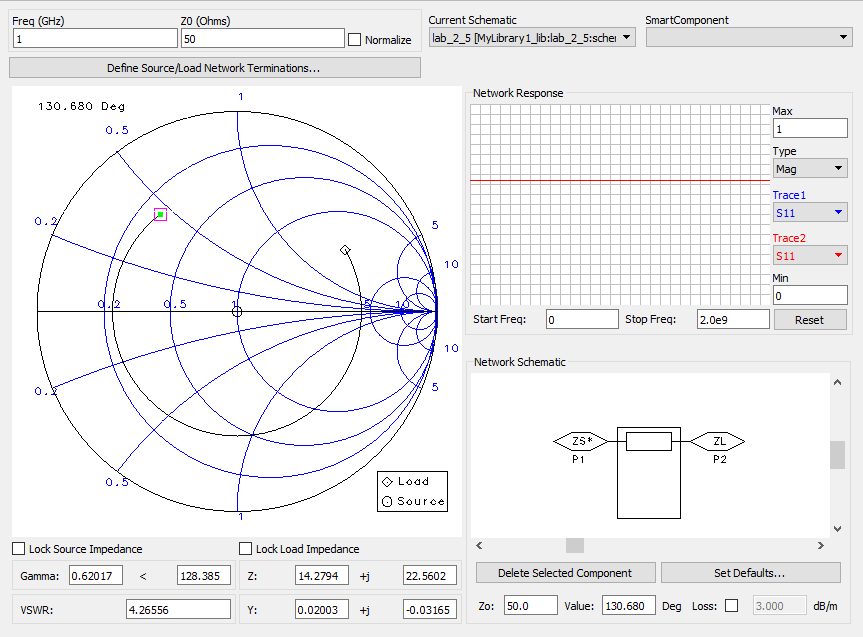
\includegraphics[width=0.8\linewidth,frame]{../Figures/scu.png}
\label{fig:scu}
\caption{Smith chart utility for determination of $Z_{in2}$}
\end{figure}
The input impedance $Z_{in2}$ is determined using the Smith chart utility in ADS. Upon entering the load impedance, reflection coefficient, port reference impedance and the electrical line length, which is, $0.363\lambda=130.68^\circ$, the input impedance represented by the red square reads $14.279+j22.56\Omega$.
\begin{equation*}
    Z_{in2}=(14.28+j22.65)\Omega
\end{equation*}

\subsubsection*{Validation by circuit simulation}
\widthFigure[0.9]{lab_2_e_ckt}{Schematic for comparing calculated impedance and reflection coefficients}

\widthFigure[0.65]{lab_2_e_mag}{Magnitude of S\textsubscript{11}, S\textsubscript{22}  vs Frequency}
\widthFigure[0.65]{lab_2_e_phase}{Phase (deg) of S\textsubscript{11}, S\textsubscript{22}  vs Frequency}
\widthFigure[0.6]{lab_2_e_11_ri}{Real and imaginary parts of impedance $Z_{in1}$ vs Frequency}
\widthFigure[0.6]{lab_2_e_22_ri}{Real and imaginary parts of impedance $Z_{in2}$ vs Frequency}

\widthFigure[0.6]{lab_2_e_smith}{Real and imaginary parts of impedance $Z_{in2}$ vs Frequency}
\end{document}